\section{\textit{Service discovery}}

\textit{Service discovery} adalah proses mencari layanan yang tersedia dan relevan untuk permintaan tertentu berdasarkan deskripsi semantik fungsional dan non-fungsional. \parencite{klusch2014servicediscovery}. \textit{Servie discovery} merupakan masalah yang sangat penting untuk menyelesaikan masalah konfigurasi. \textit{Service discovery} memungkinkan perangkat dan layanan untuk saling menemukan satu sama lain, mengatur diri, dan berkomunikasi dengan lancar. Namun, seringkali \textit{service discovery} tidak dimanfaatkan secara baik sehingga menghabiskan waktu untuk mencari layanan secara aktif dan mengatur perangkat dan program secara manual. Terkadang, konfigurasi layanan memerlukan keahlian khusus lainnya yang tidak berhubungan dengan apa yang ingin dicapai, sehingga hal ini membuat proses menjadi terhambat. Service discovery membantu untuk mengatasi masalah ini dengan membuat proses ini lebih otomatis dan mudah dilakukan \parencite{ServiceDiscovery}.

Dalam pengaplikasiannya terdapat beberapa \textit{pattern} yang dapat diaplikasikan dalam implementasi \textit{service discovery}. Menurut \parencite{micoservicearchitecture}, terdapat lima \textit{pattern} yang dapat digunakan ketika mengimplementasikan \textit{service discovery} yaitu \textit{3rd Party Registration, Client Side Serivce, Self Registration, serta Server-side service discovery}. Masing masing \textit{pattern} memiliki keunggulan dan kegunaan khusus sehingga perlu dipahami fungsi dari setiap \textit{pattern}.

\subsection{\textit{3rd Party Registration}}
\textit{3rd Party Registration pattern} adalah solusi yang digunakan pada kasus ketika service dapat di-\textit{register} dan \textit{unregister} pada \textit{registar} atau \textit{provider} nya. Solusi ini mewajibkan untuk melakukan registrasi kepada \textit{registar} ketika layanan baru dinyalakan dan melakukan \textit{unregister} ketika layanan dimatikan. layanan \textit{3rd party} yang bertanggung jawab sebagai \textit{registar} untuk mengelola hal ini \parencite{3rdpartyintegration}. Beberapa \textit{tools} yang telah menyediakan sistem layanan seperti ini yaitu \textit{Netflix Prana} yang akan bertindak sebagai \textit{side car} untuk aplikasi non-\textit{JVM} seperti Eureka ataupun AWS \textit{autoscaling groups} yang akan secara otomatis untuk meregister dan menghilangkan EC2 instance pada \textit{load balancer} nya.

Keuntungan untuk menggunakan \textit{pattern} ini ialah proses pembuatan kode yang mudah karena bergantung kepada \textit{3rd party} untuk proses registrasinya. Serta layanan \textit{3rd party} pun akan bertanggung jawab untuk melakukan pengecekan secara berkala agar sistem terus aktif sehingga meningkatkan \textit{availabilty} sistem. Namun, terdapat beberapa kekurangan diantaranya layanan \textit{3rd party} ini hanya bisa untuk melakukan \textit{discovery} secara umum. Seringkali dibutuhkan suatu solusi spesifik yang menjawab permasalahan khusus yang tidak bisa hanya diselesaikan dengan solusi seperti ini, perlu dibuat solusi \textit{custom} yang dapat menambah komponen baru ataupun arsitektur lain yang dapat menyelesaikan masalah tersebut \parencite{3rdpartyintegration}.

\subsection{\textit{Client Side}}
\textit{Client Side pattern} adalah suatu solusi \textit{service discovery} dengan proses \textit{client} yang mencari lokasi \textit{service} yang ingin dituju. \textit{Client} akan mencari lokasi dari tujuan dengan cara melakukan \textit{query} ke \textit{service registry} sehingga lokasi dari \textit{service} yang dituju dapat ditemukan secara dinamis dan \textit{runtime}. Beberapa keunggulan dari \textit{pattern} ini adalah mengurangi kompleksitas dan latensi karena mengurangi jumlah \textit{node} yang perlu di kunjungi. Namun salah satu kekurangannya yaitu meningkatnya kompleksitas kode yang dibuat, karena proses pencarian \textit{service} diletakkan di \textit{client} maka proses pencarian dan perubahan sepenuhnya dibebankan pada \textit{client}. Hal ini membuat proses pencarian tidak \textit{scalable} dan sulit ketika akan melakukan perubahan \parencite{clientsidediscovery}. Visualisasi dari \textit{client side service discovery} dapat dilihat pada \textbf{Gambar \ref{fig:client-side-discovery}}

\begin{figure}[h]
  \centering
  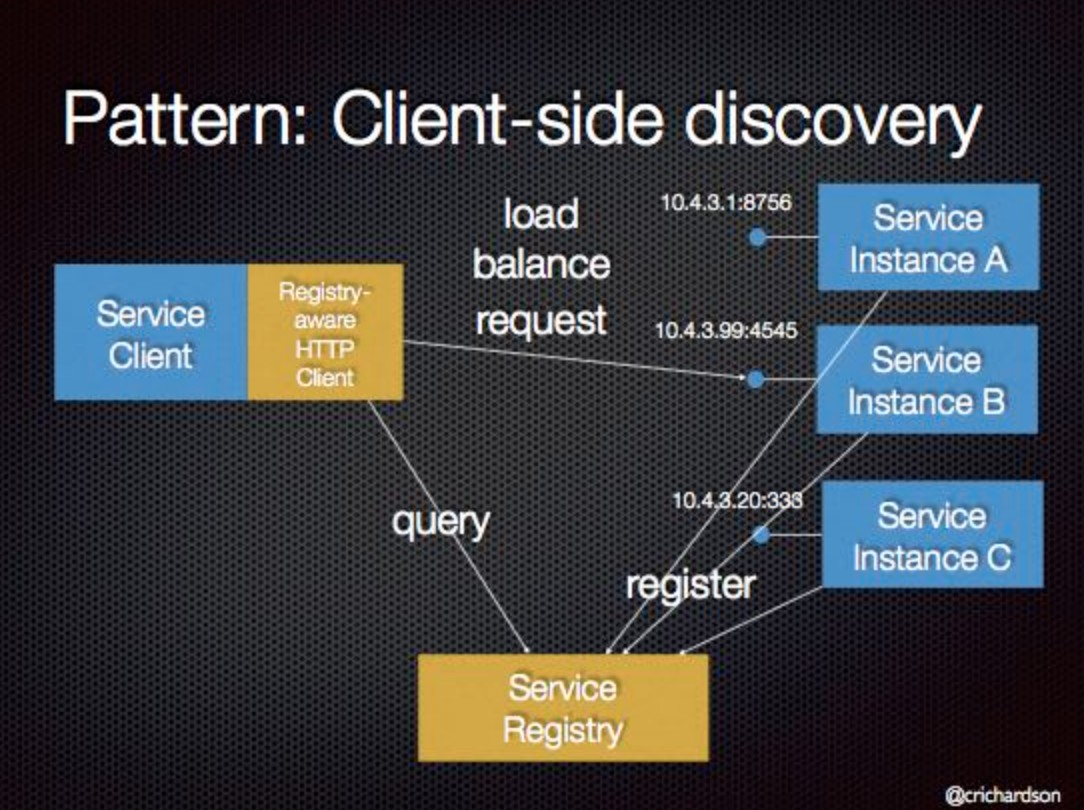
\includegraphics[width=1\textwidth]{resources/chapter-2/client-side-discovery.jpg}
  \caption{Visualisasi \textit{client side discovery} \parencite{clientsidediscovery} }
  \label{fig:client-side-discovery}
\end{figure}

\subsection{\textit{Self Registration}}
\textit{Pattern self registration service discovery} merupakan \textit{pattern} yang mudah untuk dilakukan. Pada dasarnya \textit{pattern} ini mirip dengan \textit{3rd party registration} yaitu sistem akan meregister \textit{service} ketika service dinyalakan dan \textit{service} akan di-\textit{unregister} ketika dimatikan. Meskipun solusi ini sederhana namun terdapat dua halangan diantaranya

\begin{enumerate}
  \item \textit{service} yang \textit{crash} harus dapat di-\textit{unregister} dari \textit{registry}
  \item \textit{service} yang sedang tidak bisa melayani permintaan harus di-\textit{unregister} dari \textit{registry} untuk menghindari terjadinya \textit{crash}
\end{enumerate}

Selain itu \textit{client} juga harus melakukan poling untuk mendapatkan data terbaru mengenai \textit{service} yang sedang aktif dan dapat menerima permintaan \parencite{selfregistration}.

\subsection{\textit{Server-side}}
Solusi ini memiliki visualisasi yang sama dengan \textit{client side discovery} pada \textbf{Gambar \ref{fig:client-side-discovery}}. Perbedaan yang mencolok yaitu alih alih \textit{client} yang melakukan request ke \textit{service registry}, \textit{client} akan melakukan \textit{request} kepada \textit{load balancer} dan \textit{load balancer} lah yang akan melakukan pencarian layanan mana yang sedang aktif dan dapat menerima permintaan. Cara ini merupakan cara yang paling umum digunakan untuk melakukan \textit{scaling} pada \textit{service} \parencite{servicesidediscovery}.
